\documentclass[11pt]{scrartcl}
\usepackage{graphicx}
\graphicspath{{./}}
\usepackage[sexy]{evan}
\usepackage[normalem]{ulem}
\usepackage{hyperref}
\usepackage{mathtools}
\hypersetup{
    colorlinks=true,
    linkcolor=blue,
    filecolor=magenta,      
    urlcolor=cyan,
    pdfpagemode=FullScreen,
    }
\usepackage[most]{tcolorbox}
\renewcommand{\dangle}{\measuredangle}

\renewcommand{\baselinestretch}{1.5}

\addtolength{\oddsidemargin}{-0.4in}
\addtolength{\evensidemargin}{-0.4in}
\addtolength{\textwidth}{0.8in}
% \addtolength{\topmargin}{-0.2in}
% \addtolength{\textheight}{1in} 


\setlength{\parindent}{0pt}

\usepackage{pgfplots}
\pgfplotsset{compat=1.15}
\usepackage{mathrsfs}
\usetikzlibrary{arrows}

\title{Miscellaneous Combinatorics}
\author{Azzam Labib (IG: haxuv.world)}
\date{G3-4 | 16 May 2024}
\begin{document}
\maketitle

\begin{enumerate}
    \item There are 5 steps to a flight or stairs. Aurhel can take 1 or 2 steps up at a time. How many ways are there for him to do so?
    \item Freya bought an ice cream. It costs him 40 cents. He realizes that the ice cream seller only accepts coins of 25 cents, 10 cents, and 5 cents. In how many ways can Tyler pay for the ice cream?
    \item In Newton's Balls-in-the-Bucket Challenge game, you score points by throwing balls into buckets. You have to throw 3 balls each time. If you miss, or if the ball bounces out, you score 0 for that ball. In how many ways can you score 9 points?
    \begin{figure}[h]
        \centering
        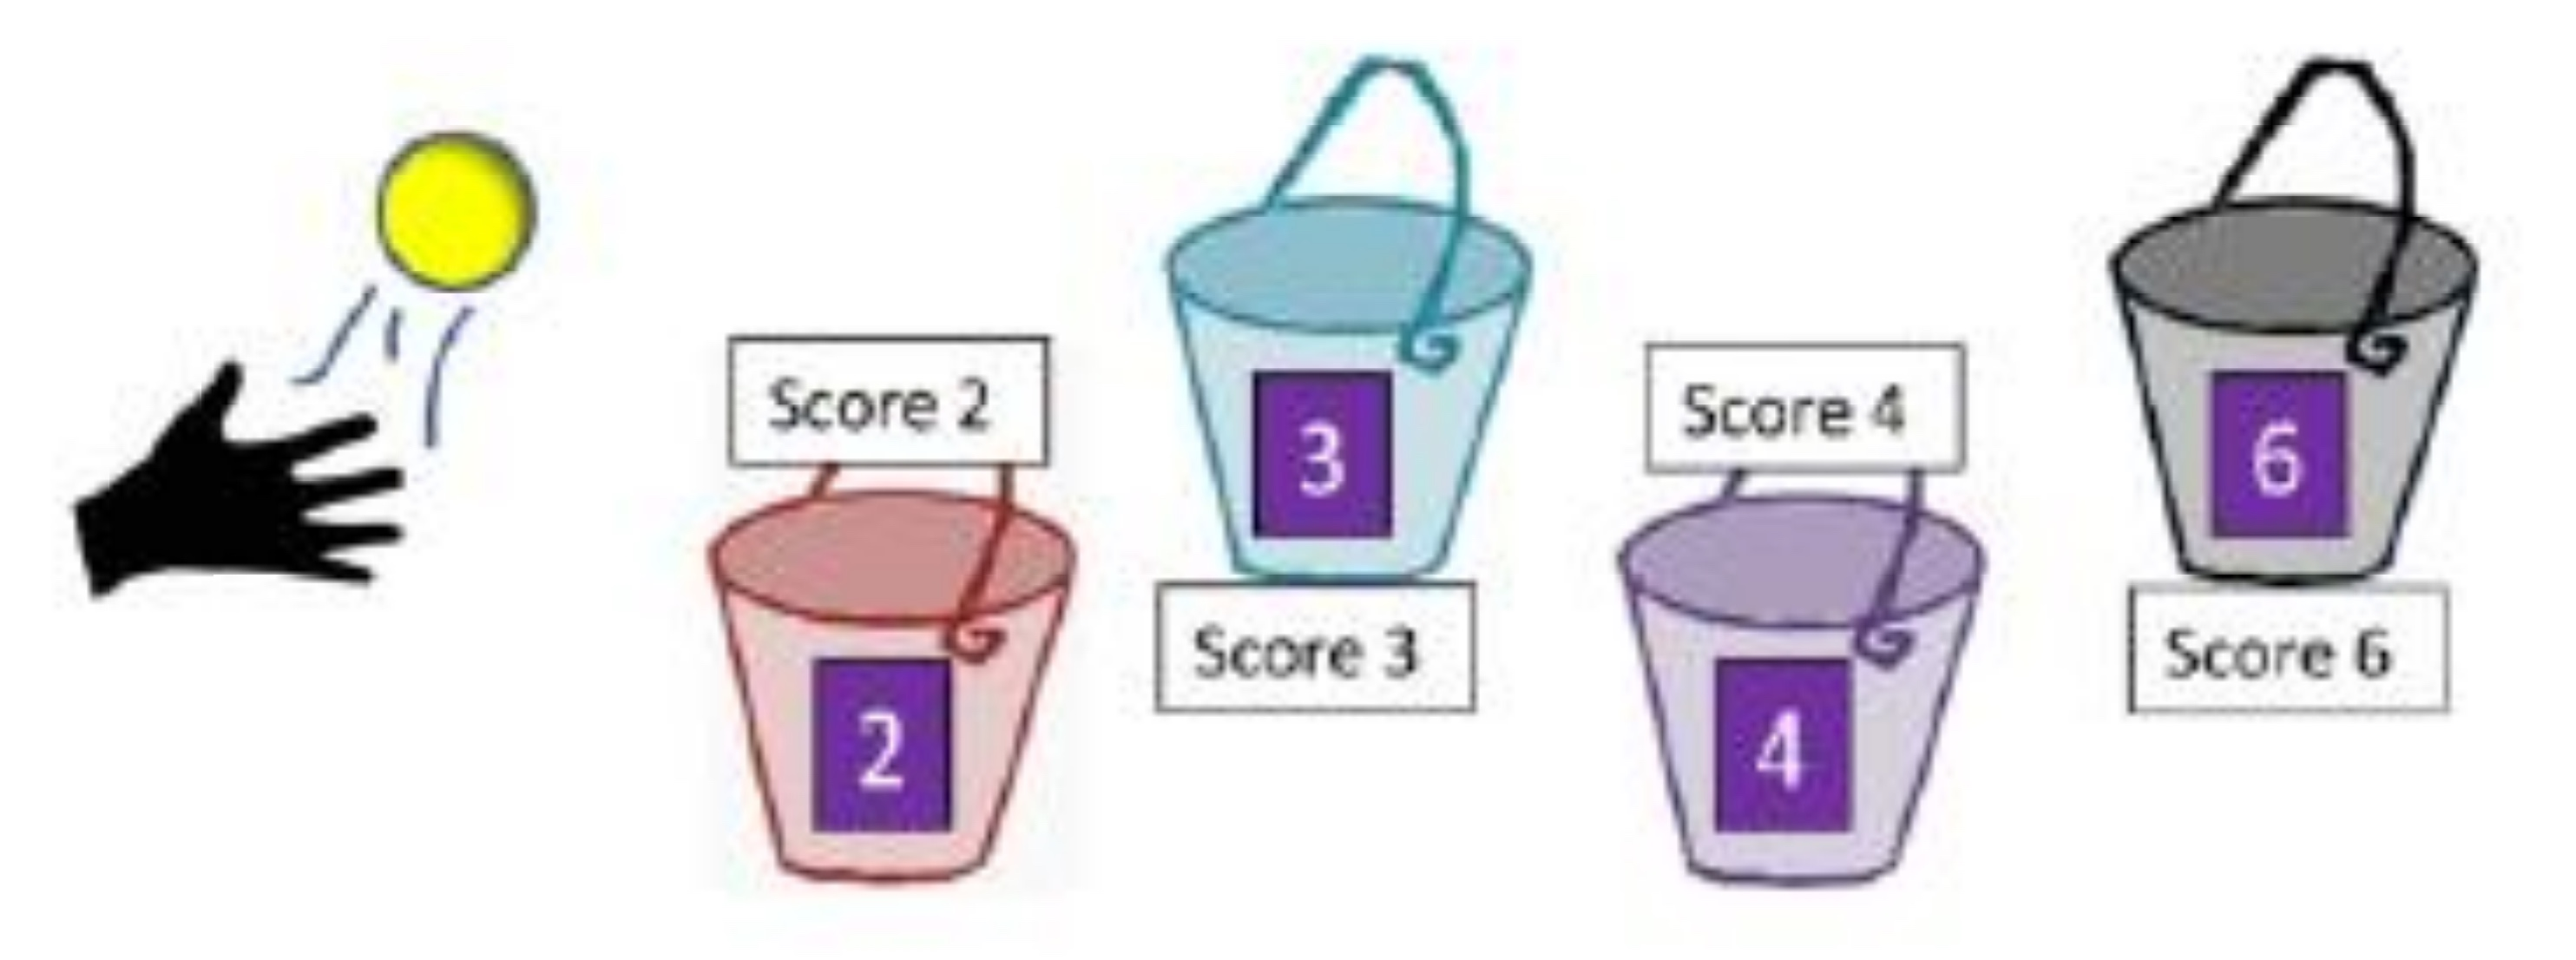
\includegraphics[width=0.5\textwidth]{StarGen/0Figure/ball-buckets-game.jpeg}
    \end{figure}
    \item Captain Olla is going to climb a mountain. There are different paths he can take to climb the mountain. He must always start at the red cross and travel upwards following the lines and dots. One of his routes has been marked with a red dashed line. This route is: right, left, left, right In how many different ways can he climb the mountain besides?
    \begin{figure}[h]
        \centering
        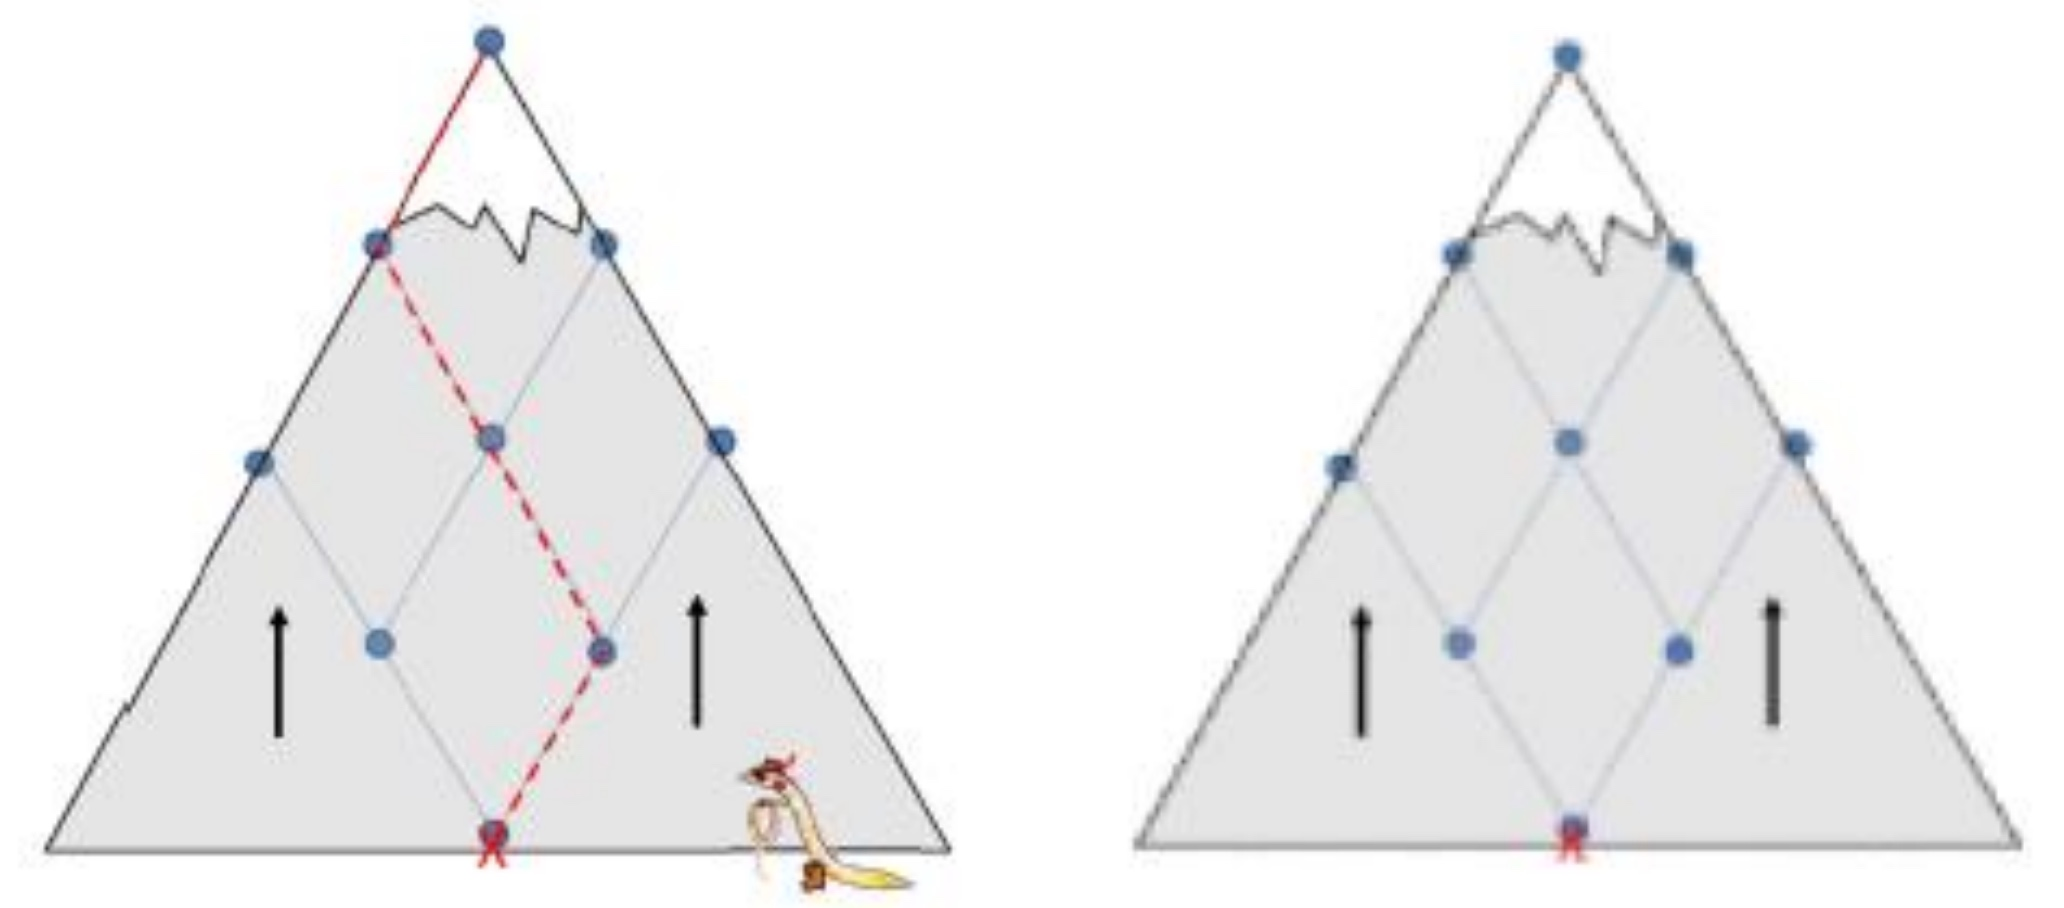
\includegraphics[width=0.5\textwidth]{StarGen/0Figure/mountain-climb-combin.jpeg}
    \end{figure}
    \item How many ways are there to arrange the blocks in a row?
    \begin{figure}[h]
        \centering
        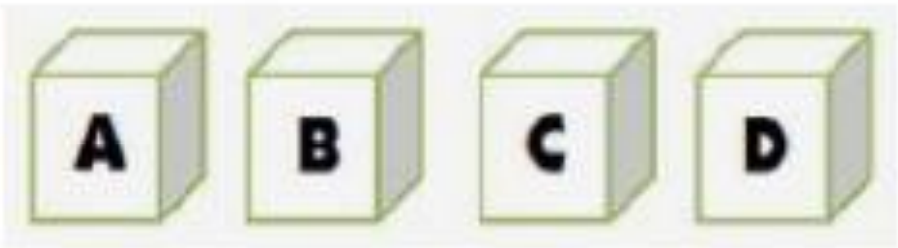
\includegraphics[width=0.5\textwidth]{StarGen/0Figure/block-abcd.png}
    \end{figure}
    
    \item In how many ways can the letters of the word "ASSESS" be arranged, all at a time?
    
    \item Given figure of the paths of the running race where each letter represent checkpoint. Each participants starting from the left (letter "N") running to the right until the finish (letter "A") on the rightmost of the figure. If they completed the race, the checkpoints they have passed will formed word "NAYLA". In how many ways are there to form the word "NAYLA"?
    \begin{figure}[h]
        \centering
        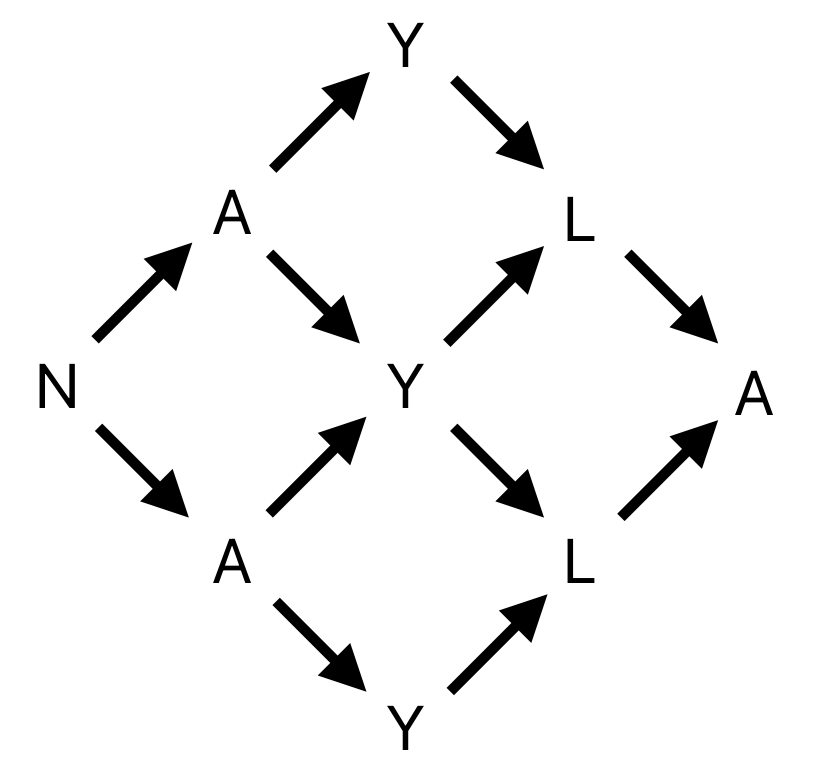
\includegraphics[width=0.5\textwidth]{StarGen/0Figure/running-race-nayla.png}
    \end{figure}
    
    \item You are going on a hike. You can choose 1 jacket and 1 hat. How many outfits can you choose from?
    \begin{tcolorbox}[colback=red!10,colframe=red!75!black]
    Jacket: blue, green, pink, yellow
    \end{tcolorbox}
    \begin{tcolorbox}[colback=blue!10,colframe=blue!75!black]
    Hat: purple, orange, black, red
    \end{tcolorbox}
    
    \item In how many ways can 5 people line up if two of the people refuse to stand next to each other?
    \item If 5 students are playing musical chairs where the chairs are arranged in a circular shape, how many ways can the 5 students sit?
    \item Five kids race during the sports festival, and the school will award the first 3 kids who won the race, regardless of the order. Assuming there's no tie, how many possible group winners are there?
    \item Oline and Erine play "Just Dice" where they only guessing each other number on the dice. Each of them rolls a dice in their turn in turn. Oline get the first turn followed by Erine.
    \begin{figure}[h]
        \centering
        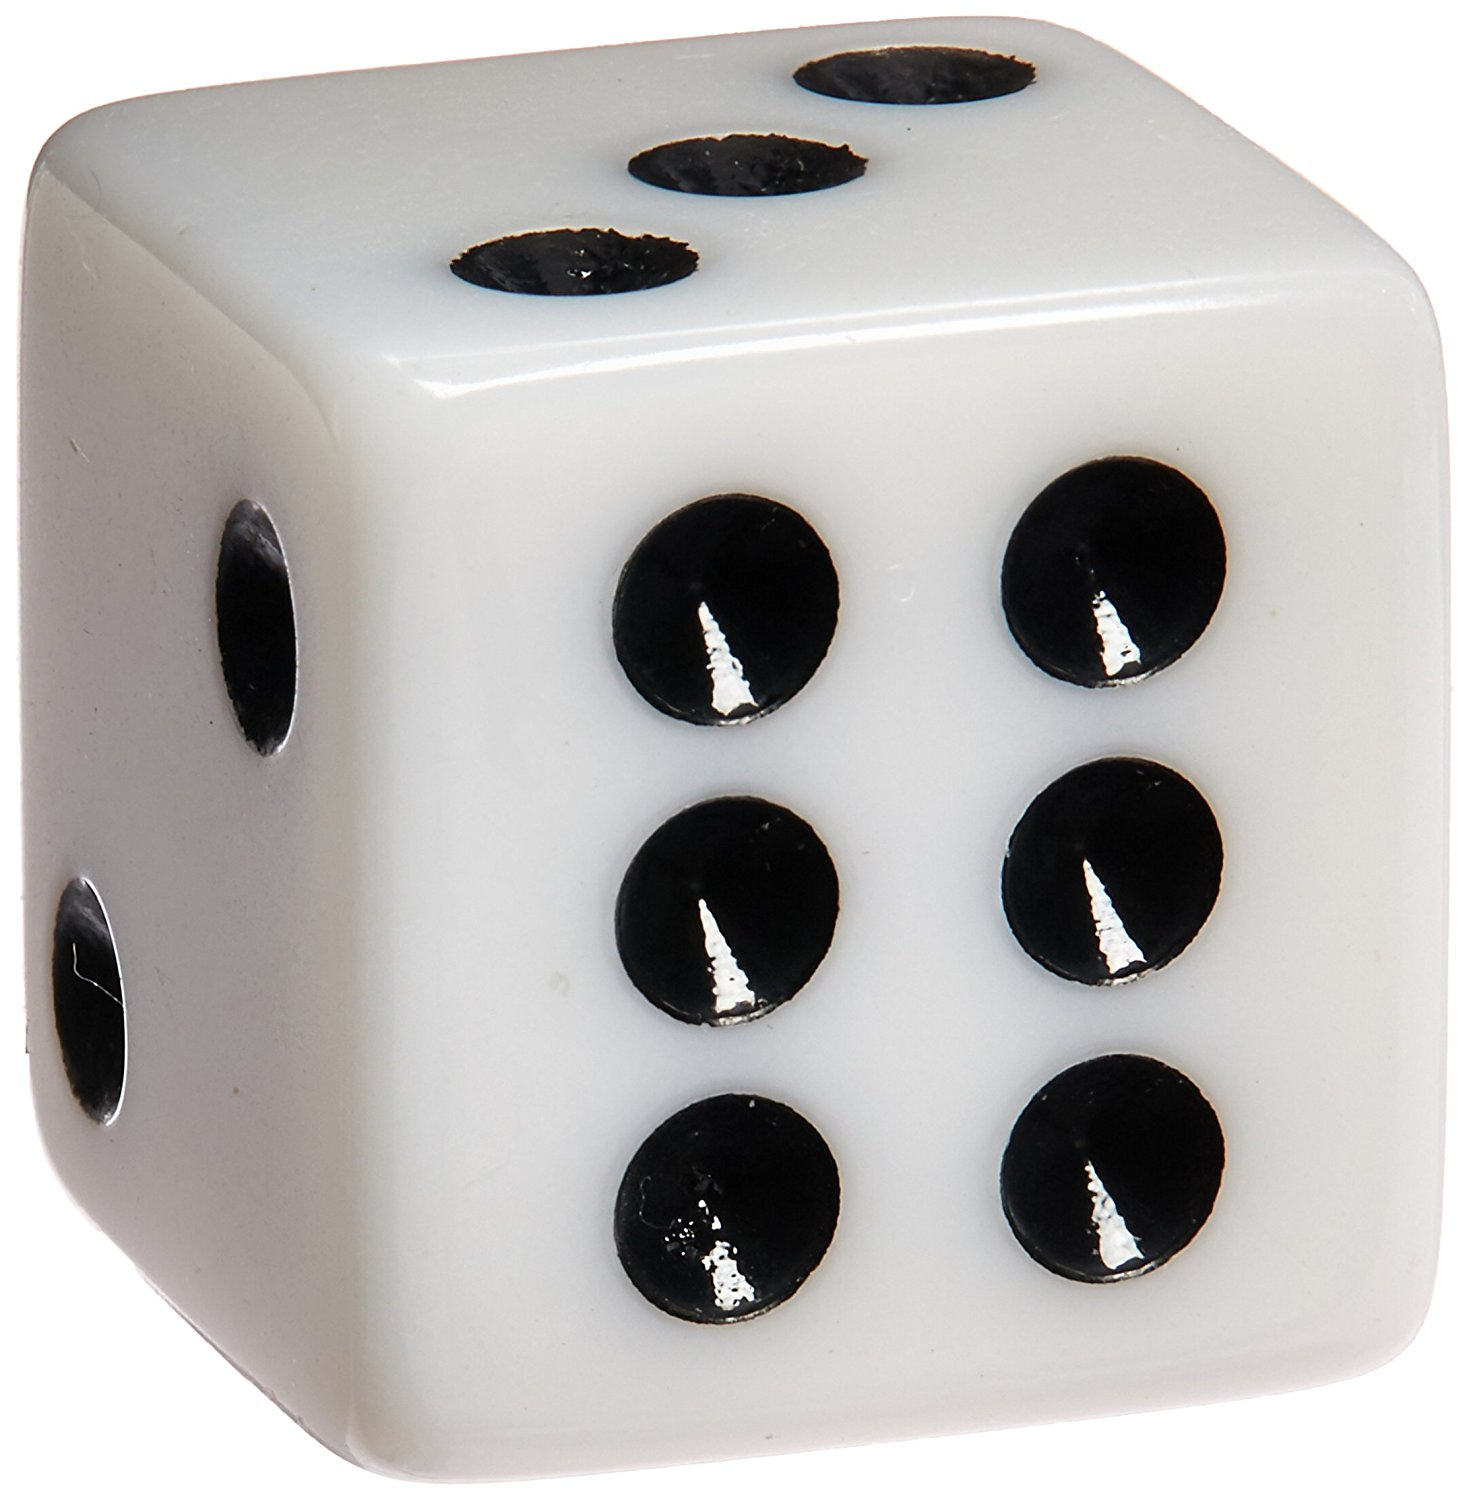
\includegraphics[width=0.2\textwidth]{StarGen/0Figure/dice-1.jpg}
    \end{figure}
    \begin{enumerate}[a)]
        \item What is the probability that Oline get 1 on the dice?
        \item What is the probability that Erine get an even number on the dice?
        \item What is the probability that Oline get 2 and right after that Erine get 3 on the dice?
        \item What is the probability that Oline get an odd number and right after that Erine get a prime number on the dice?
    \end{enumerate}

    
    \item You just completed a 10-question true or false quiz and scored 80 out of 100. How many questions can you answer differently while still maintaining a score of 80 out of 100?
\end{enumerate}

\end{document}